En este capítulo, se describen las tecnologías y conceptos asociados al proyecto, comenzando con la descripción del Sistema Operativo \textit{Android}, posteriormente se da paso a explicar claramente el paradigma de el Internet de las Cosas. Finalmente, se realiza una revisión al estado del arte relativo a sistemas similares de gestión de filas de atención que existen en la actualidad.\\

\subsection{Tecnologías Asociadas}
\subsubsection{Android}

\textit{Android} es un sistema operativo basado en un \textit{kernel} de \textit{Linux}, su interfaz de usuario está basada en la manipulación directa por pantalla táctil, diseñado para teléfonos inteligentes y \textit{tablets}. El sistema operativo utiliza el ingreso tactil para simular acciones del mundo real, como arrastrar, pinchar y presionar para manipular objetos en pantalla. Sin embargo, ha sido incorporado a otros dispositivos como: televisores, cámaras digitales, consolas de videojuegos, entre otros.\\

El sistema operativo fue desarrollado por la empresa \textit{Android Inc.}, una firma comprada por \textit{Google} el año 2005. \textit{Android} se desarrolla de forma abierta, a diferencia de \textit{iOS} o \textit{Windows Phone}, y se puede acceder al código fuente y también a la lista de incidencias donde se pueden ver los problemas no resueltos y reportar nuevos.\\

Desde el año 2011 \textit{Android} tiene la mayor cantidad de instalaciones en dispositivos móviles, y desde el 2013 estos dispositivos se venden más que todos sus competidores combinados \cite{Bus14}. En julio del mismo año su tienda de aplicaciones, \textit{Google Play}, alcanzo el millón de aplicaciones publicadas, y más de 50 mil millones de aplicaciones descargadas \cite{Pho13}. Una encuesta de desarrolladores realizada entre abril y mayo del 2013 concluyó que el 71\% de los desarrolladores de aplicaciones móviles desarrolla para \textit{Android} \cite{Dev13}. En la Tabla 1 se pueden apreciar las versiones de \textit{Android} a las que Google brinda soporte en la actualidad, su nombre clave, su fecha de lanzamiento y penetración de mercado en el total de dispositivos al 5 de Febrero del 2015.\\


\begin{spacing}{1.0}
\begin{table}[H]
\centering
\caption{Versiones de Android soportadas por Google en la actualidad \cite{And15}.} 
\begin{tabular}{|c|c|c|c|c|}
\hline 
\rowcolor{gray!30} &&&&\\
\rowcolor{gray!30} \textbf{Versión} & \textbf{API} & \textbf{Nombre Clave} & \textbf{Fecha de}  & \textbf{Distribución}\\ 
\rowcolor{gray!30}  \textbf{} & \textbf{} & \textbf{} & \textbf{lanzamiento} & \textbf{}\\[0.3cm]
\hline 
&&&&\\[-0.2cm]
5.0 & 21 & Lollipop & 25 de Junio, 2014 & 1.6\%\\
\hline 
&&&&\\[-0.2cm]
4.4 & 19 & KitKat & 31 de Octubre, 2013 & 39.7\%\\
\hline 
&&&&\\[-0.2cm]
4.3 & 18 & Jelly Bean & 24 de Julio, 2013 & 6.3\%\\
\hline
&&&&\\[-0.2cm]
4.2 & 17 & Jelly Bean & 13 de Noviembre, 2012 & 19.8\%\\
\hline
&&&&\\[-0.2cm]
4.1 & 16 & Jelly Bean & 9 de Julio, 2012 & 18.4\%\\
\hline
&&&&\\[-0.2cm]
4.0.3 - 4.0.4 & 15 & Ice Cream Sandwich & 16 de Diciembre, 2011 & 6.4\%\\
\hline
&&&&\\[-0.2cm]
2.3.3 - 2.3.7 & 10 & Gingerbread & 9 de Febrero, 2011 & 7.4\%\\
\hline
&&&&\\[-0.2cm]
2.2 & 8 & Froyo & 20 de Mayo, 2010 & 0.4\%\\
\hline
\end{tabular}
\label{tabla_GCM}
\end{table}
\end{spacing}



En cuanto al desarrollo de aplicaciones para \textit{Android} habitualmente se implementan en el lenguaje de programación \textit{Java}, utilizando alguno de los siguientes entornos de desarrollo: \textit{Android Software Development Kit (Android SDK)} o \textit{Android Software Development Kit (Android Studio)}. También se pueden usar otros lenguajes y herramientas de desarrollo como \textit{Visual Basic} utilizando el \textit{SDK Basic4Android}. Además se puede utilizar C\#, .NET. Para estos últimos lenguajes se pueden usar los \textit{SDK Visual Studio}, \textit{MonoDevelop} o \textit{Xamarin Studio}.\\ 

Android SDK es un conjunto de herramientas de desarrollo de aplicaciones para \textit{Android}. Esta incluye un \textit{debugger}, librerías, un emulador de dispositivo, documentación, código de ejemplo y tutoriales para apoyar el desarrollo, además de incluir en la actualidad el entorno de desarrollo integrado \textit{Eclipse}. Estas herramientas se pueden utilizar en sistemas basados en \textit{Microsoft Windows}, \textit{Mac OSX} y Linux.\\

\subsubsection{\textit{Google Cloud Messaging} para \textit{Android}}

GCM \textit{(Google Cloud Messaging)} es un servicio gratuito de mensajería, que permite el envío de notificaciones desde un servidor a una aplicación \textit{Android}. Puede tratarse de un mensaje corto que indique un mensaje sencillo. Los mensajes tienen un tamaño de hasta 4 KB de datos \cite{And14}.\\
GCM reemplaza a la versión beta de C2DM, anterior servicio de mensajería nube – dispositivo de \textit{Android}. C2DM está obsoleto, y ya no está en funcionamiento para aplicaciones nuevas.\\

\myparagraph{Arquitectura}

GCM esta compuesto por un servidor de conexión proporcionado por Google (GCM Connection Servers), un servidor 3rd – Party App Server que interactúa con el servidor de conexión y una aplicación cliente \textit{(Client App)} que se ejecuta en el dispositivo Android. La estructura de la arquitectura antes descrita se puede ver en la Figura 1.\\

\begin{figure}[H]
\centering
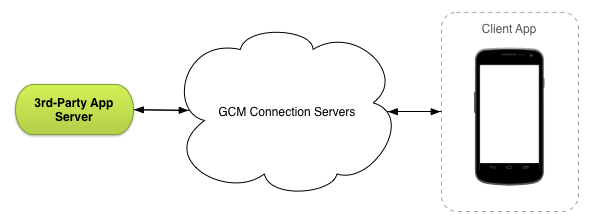
\includegraphics[scale=0.65]{images/capitulo2/GCM_arquitectura.png}
\caption{Arquitectura de GCM \cite{And14}.}
\label{iot}
\end{figure}

En la Tabla2, se detalla cada uno de los componentes de la arquitectura de GCM mostrados en la Figura1.\\


\begin{spacing}{1.0}
\begin{table}[H]
\centering
\caption{Componentes de GCM} 
\begin{tabular}{| >{\arraybackslash\columncolor{gray!30}}p{3.1cm}| >{\arraybackslash}p{10.4cm}|}
\hline 
\multicolumn{2}{| >{\arraybackslash\columncolor{gray!30}}c|}{}\\[-0.2cm]
\multicolumn{2}{| >{\arraybackslash\columncolor{gray!30}}l|}{\textbf{Componentes}}\\[0.2cm]
\hline 
&\\[-0.2cm]
\textbf{Client App} & La aplicación es ejecutada sobre un dispositivo \textit{Android}. El dispositivo debe contar con \textit{Android} 2.2 y debe tener iniciada una sesión con su cuenta de \textit{Google}. \\
\hline 
&\\[-0.2cm]
\textbf{3rd-Party Application Server} & Es un servidor (es implementado por programadores que deseen utilizar el servicio de GCM) que envía datos a una aplicación \textit{Android} en un dispositivo a través del servidor GCM.\\
\hline 
&\\[-0.2cm]
\textbf{GCM Connection Servers} & Son servidores que provee \textit{Google}, y se encargan de recibir los mensajes desde el servidor \textit{3rd-Party Application} y enviarlos al dispositivo \textit{Android} donde se encuentra la aplicación cliente \textit{(Client App)}.\\
\hline
\end{tabular}
\label{tabla_componentesGCM}
\end{table}
\end{spacing}

\myparagraph{Enviar Mensajes}

A continuación se muestra la secuencia general de eventos que ocurren cuando nuestro servidor envía un mensaje:

\begin{enumerate}
\item Nuestro servidor (3rd-Party Application) envía el mensaje a los servidores GCM de Google.
\item Google guarda el mensaje en una cola de espera en caso de que el dispositivo Android esté offline.
\item Cuando el dispositivo Android está online, Google le envía el mensaje.
\item En el dispositivo Android, el sistema se encarga de que el mensaje  sea recibido por la aplicación correcta utilizando los permisos correspondientes. Lo anterior despierta a la aplicación Android implicada. La aplicación no necesita estar ejecutándose para recibir el mensaje.
\item La aplicación Android procesa el mensaje.
\end{enumerate}

\myparagraph{Recibir Mensajes}

Esta es la secuencia de eventos que ocurren cuando una aplicación Android instalada en un dispositivo móvil recibe un mensaje:
\begin{enumerate}
\item El sistema recibe el mensaje entrante y extrae una API key junto con los datos del mensaje.
\item El sistema pasa la API key y los datos a la aplicación correspondiente.
\item La aplicación extrae los datos asociados a la API key y procesa la información contenida.
\end{enumerate}

\subsubsection{Notificaciones Push}

La tecnología \textit{Push}, es un estilo de comunicación sobre internet donde la petición de una transacción comienza en el servidor.\\ 

Los servicios \textit{Push}, generalmente, están basados en información a medida. Es decir, funcionan bajo un modelo publicador – suscriptor. Un cliente se suscribe  a un medio de comunicación y, cuando haya nuevo contenido disponible el servidor deberá enviar la información al usuario.\\ 

La mensajería Push presenta dos ventajas:

\begin{enumerate}
\item La notificación es instantánea, los mensajes se reciben de inmediato.
\item Las notificaciones \textit{Push}, no necesitan que la aplicación receptora esté ejecutándose en el dispositivo y realizando consultas al servidor consultando por nueva información. Esto permite que la aplicación se esté ejecutando en segundo plano y se active cuando reciba un mensaje.
\end{enumerate}

\textit{BlackBerry} fue la primera plataforma móvil que integró la tecnología \textit{Push} para el servicio de correo electrónico en sus dispositivos. En el año 2009, \textit{Apple} lanzó su propia infraestructura de notificaciones mediante tecnología \textit{Push}, a través de APNs (\textit{Apple Push Notification service)} . La última plataforma en incorporar éste servicio fue \textit{Android} a través de C2DM \textit{( Cloud to Device Messaging)} de \textit{Google}. Dicha tecnología se encarga de la gestión de cola y envío de mensajes a la aplicación cliente. Hace poco tiempo \textit{Google} actualizó su plataforma de notificaciones. Ahora se llama GCM \textit{(Google Cloud Messaging)} que sustituye a C2DM. Los requisitos para los dispositivos móviles que quieran utilizar la infraestructura son disponer una versión de \textit{Android} 2.2 o superior y tener instalado \textit{Google Play}. Estos mensajes se muestran en nuestro dispositivo por ejemplo cuando recibimos un mensaje SMS o tenemos una llamada perdida. Constan de un \textbf{icono} y un \textbf{texto} que se muestra en la barra de estado de \textit{Android} junto con un \textbf{mensaje} descriptivo y una marca que contiene la \textbf{hora} en que llegó la notificación. A modo de ejemplo, cuando tenemos una notificación de alguna aplicación en nuestra barra de estado, por un lado vemos el icono junto a un texto principal y más abajo un segundo texto con un mensaje de carácter descriptivo; lo anterior, se puede apreciar en la Figura2.\\

\begin{figure}[H]
\centering
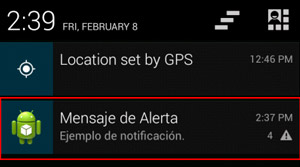
\includegraphics[scale=0.65]{images/capitulo2/notificacionPush.jpg}
\caption{Ejemplo de Notificación Push en Android. \cite{Sgo11g}.}
\label{notificacionPush}
\end{figure}


\subsubsection{Web Service}

Un servicio web ( \textit{Web Service} en Inglés ) es una tecnología que utiliza un conjunto de protocolos y estándares que sirven para intercambiar datos entre aplicaciones. Éstas aplicaciones pueden estar desarrolladas en diferentes lenguajes, o pertenecer a plataformas distintas. Para poder intercambiar información a través de redes de computadores se utilizan los servicios web. Éstos servicios aportan interoperabilidad entre aplicaciones, es independiente de las plataformas en donde estén instaladas. Permiten que software de diferentes compañías, ubicadas en distintas partes del mundo, puedan ser combinados y proveer servicios integrados.\\

A modo de ejemplo, la Figura 3 corresponde a un esquema donde las flechas rojas indican el flujo de datos ante una \textbf{solicitud} de una aplicación \textit{Android} a una base de datos MySQL, realizada a través de un web service escrito en \textit{PHP} y el respectivo flujo de datos de \textbf{respuesta}, flechas verdes, enviados desde la base de datos hacia la aplicación móvil utilizando el formato de intercambio de datos JSON.\\

\begin{figure}[H]
\centering
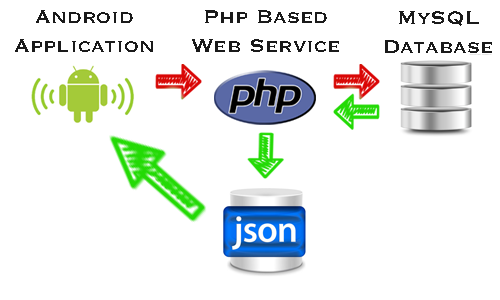
\includegraphics[scale=0.65]{images/capitulo2/webServiceJSON.png}
\caption{Flujo de datos entre una aplicación \textit{Android}, \textit{Web Service PHP} y MySQL. \cite{Myb13}.}
\label{webService}
\end{figure}

\subsubsection{MySQL}
Es un sistema de gestión de base de datos relacional. MySQL\footnote{http://www.mysql.com/} es utilizado en aplicaciones web y de escritorio. Sin embargo se puede conectar con aplicaciones móviles mediante el uso de \textit{Web Service}. Es uno de los sistemas de bases de datos de código abierto más populares, existe bastante documentación sobre cómo conectar MySQL con: servidores web y servicios web escritos en diversos lenguajes de programación, además de librerias que soportan la comunicación con aplicaciones para varias: plataformas y lenguajes de programación.\\

\subsection{Teoría de Colas}

Hoy en día estamos rodeados de sistemas de colas o filas de espera, cuando estamos en un taco vehicular, un semáforo mal regulado, un peaje, esperamos en el teléfono a ser atendidos por un operador, entre otros. En el sistema a desarrollar se quiere proporcionar información al cliente sobre el estado de avance de la fila donde éste solicitó un número de atención. Como por ejemplo, advertir un tiempo de atención estimado por cada cliente atendido. Para ello, es necesario considerar esta teoría en el prototipo a desarrollar.\\

La teoría de colas se dedica al estudio matemático de colas o líneas de espera dentro de un sistema. Estudia elementos como el tiempo de espera promedio o la capacidad de trabajo que tiene un sistema sin que colapse. Esta teoría es utilizada en una variedad de áreas como: telecomunicaciones, comercio, cadenas productivas, etc..\\

Un sistema de colas puede ser descrito como \textbf{clientes} que llegan a un centro en busca de un \textbf{servicio}, deben esperar si éste no es entregado de inmediato, y abandonan luego de ser atendidos. En algunos casos los clientes se retiran del sistema debido a un tiempo de espera excesivo. Son cuatro los componentes que definen la estructura básica de un sistema de colas\cite{Sch04}: 

\begin{enumerate}
\item Modelos de llegada: fijos o aleatorias según un patrón de comportamiento.
\item Modelos de servicio: fijo o definido por un tipo de distribución.
\item Disciplina de la cola: los clientes son atendidos dependiendo el orden de llegada al sistema: 
\begin{enumerate}
\item FCFS (\textit{First Coming First Served:}) El primer cliente en llegar es el primero en ser atendido.
\item LCFS (\textit{Last Coming First Served:}) El último cliente que llega es el primero en ser atendido.
\item PS (\textit{Procesor Sharing:}) Procesamiento compartido.
\end{enumerate}
\item Notación de Kendall (A/B/c/k/m) donde:
\begin{enumerate}
\item A distribución de llegadas.
\item B distribución de tiempo de servicio.
\item c número de canales de servicios.
\item k capacidad de la cola.
\item m tamaño de la población.
\end{enumerate}
\end{enumerate}

Por lo anterior se puede deducir que un sistema de colas es altamente complejo. Sin embargo, para este proyecto se considerará un modelo simple en el que habrá una fila de espera para cada canal de atención (servicios). Finalmente, se calculará el tiempo medio de espera para cada servicio. Éste, será enviado en las notificaciones a cada dispositivo cada vez que la fila de espera avance.\\


\subsection{Internet de las cosas}

El término de Internet de las cosas no es conocido por las personas que utilizan tecnología a diario: desde computadores, termostatos y teléfonos inteligentes, hasta una maleta inteligente que está dotada de GPS, y sensores que se comunican vía \textit{Bluetooth} con el celular y la red \cite{Inf14}.\\ 

Para \textit{Cisco Internet Business Solutions Group}, el gigante mundial en infraestructura de red, lo define como ``simplemente es el punto en el tiempo donde comenzaron a haber más 'cosas u objetos' conectadas a Internet que personas \cite{Cis11}.''\\

También se puede entender este concepto pensando en la capacidad que tiene un objeto o cosa inteligente que puede comunicarse con las personas. Este es un escenario donde animales, personas y objetos están todos conectados y provistos de un identificador único que permite que sus datos sean almacenados en un sistema. De esa forma, podemos acceder a los datos asociados a esa entidad e interactuar con ellos. Como consecuencia, existe la posibilidad de transferir datos sobre éstos a través de la red sin necesidad de interacción: persona - persona o persona - ordenador. Lo anterior es posible gracias a la evolución de las tecnologías inalámbricas e Internet.\\

Lo descrito anteriormente se puede ver en la Figura 2, donde se aprecia claramente la diversidad de objetos que son considerados en este paradigma.

\begin{figure}[H]
\centering
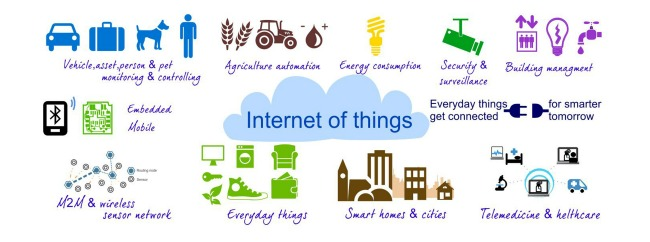
\includegraphics[scale=0.70]{images/capitulo2/lOT.jpg}
\caption{Internet de las cosas \cite{The14}.}
\label{IoT}
\end{figure}


\subsubsection{Big Data}

Los computadores y los dispositivos móviles han dejado de ser los únicos objetos capaces de comunicarse con Internet. Lo que antes era algo futurista, es ahora una realidad. Automóviles, electrodomésticos y otros objetos nunca imaginados ahora también se pueden conectar a la red. Y con su masificación, nuevos productos y servicios irán surgiendo conforme a las posibilidades tecnológicas se perfeccionen.\\

Esta unión entre el mundo de las cosas y el mundo virtual representará un incremento vertiginoso del \textit{Big Data}. Es decir, la tecnología de procesado de millones de datos en tiempo real, provenientes de diferentes ámbitos como: negocios, gobierno, servicios financieros, medicina, ciencia e ingeniería.\\

Las soluciones tecnológicas para analizar esa cantidad abismal de datos, es clave para el desarrollo de las empresas dentro de la nueva situación de mercado de hoy en día. En este contexto, la movilidad y la nube tendrán un rol fundamental: mientras los smartphones u objetos de los consumidores, conectados a la red, emiten volúmenes importantes de información, la nube será el lugar donde se alojarán. La ventaja que brindan las soluciones análiticas radica en que las empresas podrán tomar decisiones más acertadas y ofrecer a sus clientes lo que ellos necesitan.\\

El año 2012, investigadores de IBM se unieron con la ciudad de Lyon en Francia para crear un sistema que ayude a los agentes de tráfico a reducirlo en las calles de la ciudad. El sistema \textit{Decision Support System Optimizer}, utiliza informes en tiempo real sobre el tráfico para detectar posibles tacos. De tal modo, si un agente detecta que puede haber un atasco en algún punto, puede cambiar las señales de tráfico para mantener las carreteras con un flujo constante \cite{IBM12}.\\

En el contexto del proyecto, los clientes que asisten a los centros de atención, donde existe una atención masiva de clientes en los diversos servicios que proporcionan, entregarán información valiosa a éstos, a través de sus dispositivos móviles, dándoles la posibilidad de tomar decisiones acertadas y oportunas para reducir los tiempos de atención en las filas de espera de los servicios más requeridos.\\

\subsection{Estado del Arte}

En este apartado, se revisarán sistemas similares al que se pretende desarrollar en el proyecto, que signifiquen un aporte parcial para su posterior implementación. Analizar estos sistemas significan un apoyo para considerar las funciones más comunes y detectar características relevantes que se pueden incluir en el proyecto.\\

\subsubsection{Banco de Venezuela, Cola Virtual}

Es un servicio implementado por el Banco de Venezuela, que permite a clientes y no clientes enviar un mensaje de texto desde su celular, mediante un sistema automatizado de administración de cola, solicitando un número de ticket, mucho antes de llegar a la oficina bancaria, para ser atendido por ventanilla. Va dirigido a personas naturales, clientes o no clientes de dicho banco.\\

Su uso no implica cobros por parte del Banco, pero se debe pagar por el costo del mensaje de solicitud de ticket al operador de telefonía. Es compatible con cualquier celular que permita enviar y recibir mensajes de texto (SMS), independiente del operador telefónico.\\ 

El proceso de petición de ticket es bastante engorroso. Hay dos formas de hacerlo, la primera es para celulares normales y la segunda para teléfonos inteligentes.\\ 


\subsubsection{WAVETEC, Sistema de Administración de Filas}

La empresa en cuestión, tiene una solución para las personas que tienen problemas como: el exceso de espera desorganizado, el tiempo de espera de los clientes son cada vez mayores, los empleados tienen momentos improductivos, sus clientes se molestan por un servicio que no es el que esperaban, es incapaz de monitorear el rendimiento de una sucursal desde diferentes lugares.\\

Sus soluciones son ideales para Bancos, Centros de Servicio en compañías de Telecomunicaciones, Instituciones Gubernamentales, Hospitales, Empresas del Retail, Aerolíneas, Embajadas u organizaciones con un alto flujo de clientes.  Wavetec ayuda a las empresas mas importantes de la industria para mejorar la experiencia del cliente alrededor del mundo. La solución integra diferentes tecnologías para seguir el estado de la fila: notificación vía SMS que el turno será llamado dentro de poco, permite a los clientes salir de las oficinas a otro lugar, visitar otros almacenes, etc. También se pueden solicitar turnos vía Web y SMS.\\

\myparagraph{Reportes en tiempo real}

El sistemas de Administración de Filas está equipado con un potente software de reportes que permitirá a las personas que toman las decisiones en las organizaciones actuar con valiosa información. Esta herramienta ha sido desarrollada para gerentes y ejecutivos para administrar el flujo de trabajo de sus áreas de servicio al cliente en cada sucursal a través de información de inteligencia de negocios, por ejemplo, tiempos de espera promedio, numero exacto de clientes en espera, tiempos de ausencia de los asesores y muchos mas indicadores de desempeño.\\

\myparagraph{Reportes de sucursales}

Se pueden resumir por 5 periodos de tiempo (por hora, día, semana, mes, año).

\begin{enumerate}
\item \textbf{Reportes Resumidos:} Muestra el rendimiento en servicio de una sucursal en un momento determinado.
\item \textbf{Reportes por Categoría:} Entrega información del flujo de clientes en cada categoría de servicio.
\item \textbf{Reportes por Operador:} Entrega información sobre el rendimiento de un operador en la sucursal.
\item \textbf{Reportes de Alertas:} Este informe compara el rendimiento de la sucursal contra los indicadores de desempeño (KPI) de tiempo de espera, tiempo de duración de la atención y la capacidad de asientos en la sala de espera.
\end{enumerate}

\subsubsection{Q-sige, Sistema Inteligente de Gestión de Esperas}

El Sistema Inteligente de Gestión de Esperas, está compuesto por diversos programas que se comunican a través de la red. Cuenta con un módulo de estadísticas (SIGEST) y un módulo de \textbf{Cita Prévia (web o Telefónica)} mediante el cual, el cliente puede reservar una hora. Permite optimizar la calidad de atención al público. Su ventaja principal es, además de reducir los tiempos de espera, transformar las incómodas filas en zonas de espera confortables para los clientes. En estas cómodas zonas de espera, se les informa a las personas cuándo y dónde se les atenderá. \cite{Idm14}.\\

Otra funcionalidad del sistema SIGE es proveer de información a los responsables de la gestión de calidad de la atención al público, aportando con información que permite conocer lo que está ocurriendo en un instante de tiempo y, reaccionar oportunamente para analizar y optimizar sus recursos.\\ 

Este sistema cuenta con dos versiones. Una versión reducida de Q-sige, diseñado para negocios pequeños con un espacio reducido. La versión completa se llama Q-sige Synergy, está orientada a empresas con un gran número de oficinas y servicios.\\




